\documentclass[../resumosTCOM.tex]{subfiles}

\newenvironment{conditions}
  {\par\vspace{\abovedisplayskip}\noindent\begin{tabular}{>{$}l<{$} @{${}={}$} l}}
  {\end{tabular}\par\vspace{\belowdisplayskip}}

\begin{document} 

Alfabeto (\(\sum\)) é um conjunto finito de símbolos não vazios.

\paragraph{}

String é uma sequência finita de símbolos selecionados do alfabeto.

\paragraph{}

Linguagem L sobre um alfabeto (\(\sum\)) é um subconjunto de \(\sum^*\) (\(L \subseteq  \sum^*\))
\begin{itemize}
    \item \(\sum^* = \sum^0 \bigcup \sum^+ = \sum^0 \bigcup \sum^1 \bigcup \sum^2 \bigcup ... \)
    \item Qualquer problema pode ser convertido numa linguagem e vice-versa.
\end{itemize}

\paragraph{}

DFA é determinista: num estado, para cada input, existe apenas uma possível transição.

\paragraph{}

DFA: \(A = (Q, \sum, \delta, q_0, F)\)
\begin{itemize}
    \item Q é um conjunto de estados.
    \item \(\sum\) é o alfabeto.
    \item \(\delta\) é a função de transição, de estados e inputs para estados.
    \begin{itemize}
        \item Exemplo: \(p = \delta(q, a)\)
    \end{itemize}
    \item \(q_0 \in Q\) é o estado inicial.
    \item \(F \subseteq Q\) é o conjunto de estados finais/de aceitação.
\end{itemize}

\paragraph{}

Diagrama de transição e respetiva tabela:
\begin{figure}[H]
    \centering
    \subfloat{{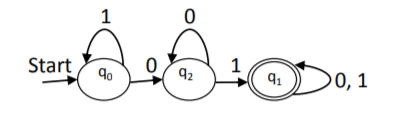
\includegraphics[width=5cm]{images/dfa.PNG} }}%
    \qquad
    \subfloat{{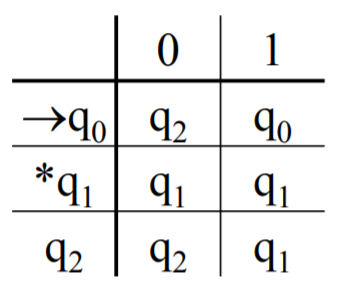
\includegraphics[width=5cm]{images/dfa_table.PNG} }}%
    \label{fig:dfa}%
\end{figure}

\paragraph{}

Se uma linguagem L é L(A) para um DFA A, então é uma linguagem regular.

\end{document}

